\section{Optimization Technique and Promotion Point Tuning}
\subsection{Optimization Technique}
Since the total exectuion happens before $P_{i,x}$ could not exceed $P_{i,x}$, we will introduce an optimization technique based on this fact.  Function $f_i(\tau_j,t',t)$ denotes the maximum resource used by $\tau_j$ during $[0,t']$, and here we denfine another function $g_i(\tau_j,t',t)$ which denotes the maximum possible resource used by $\tau_j$ during $[P_{i,x},t']$ (only if $P_{i,x}<t'$). Note that if $\tau_j$ has its index $j>i$, then 
\[
g_i(\tau_j,t',t)=0
\]
because it would never execute after $P_{i,x}$ before $J_{i,x}$ finishes.
% \subsection{$g_i(\tau_j,t',t)$  }
\begin{lemma}
If $D_j-p_j\geq C_j$, then $g_i(\tau_j,t',t)$ maximizes when $r_{j,y'}=[P_{i,x}+C_j-D_j]_0$ and all successive jobs are released as soon as possible,  as shown in Figure~\ref{fig:o1}. In this case  $r_{j,y}=r_{j,y'}+\lfloor \frac{t'-r_{j,y'}}{T_j}\rfloor T_j$.
\end{lemma}
\begin{proof}
Case 1: If $P_{i,x}+C_j-D_j\geq 0\Rightarrow r_{j,y'}=P_{i,x}+C_j-D_j$, (scenario in Figure~\ref{fig:o1}) as we shift the pattern left, $J_{j,y'}$ execution after $P_{i,x}$ will decrease linearly up to $C_j$, while  execution of $J_{j,y}$  will increase at most linearly. On the other hand, as we shift the pattern right, $g_i(\tau_j,t',t)$  would only decrease or stay the same.

Case 2 :If $P_{i,x}+C_j-D_j<0\Rightarrow r_{j,y'}=0$, as we shift the pattern left, execution of $J_{j,y'}$ decreases from $C_j$ to $0$ (when $y\neq y'$), while the increase of $J_{j,y}$ is bounded by $C_j$. On the other hand, as we shift the pattern right, $g_i(\tau_j,t',t)$  would only decrease or stay the same.
\end{proof}

\begin{figure}[h!]
 \centering
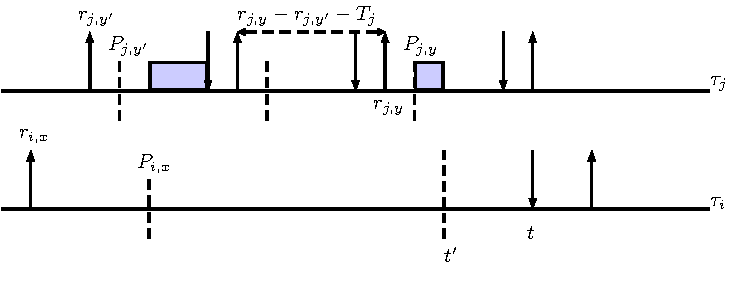
\includegraphics[scale=0.7]{fig/Cx}  
\caption{$D_j-p_j\geq C_j$}
  \label{fig:o1}
\end{figure}

With the above lemma, we have

	\begin{align}
	\begin{split}
	g_{i}(\tau_j,t',t)=
	\begin{cases}
	&\min(C_j, t'-P_{i,x})~\mbox{~~~~~~~if~} y=y'\\
	&C_j+\frac{r_{j,y}-r_{j,y'}-T_j}{T_j}C_j\\&+\min(C_j, [t'-P_{j,y}]_0)\mbox{~~~otherwise} \\
	\end{cases}
	\end{split}
	\end{align}

\begin{lemma}
If $D_j-p_j<C_j$, then $g_i(\tau_j,t',t)$ maximizes when $r_{j,y'}=[P_{i,x}-p_j]_0$ and all successive jobs are released as soon as possible,  as shown in Figure~\ref{fig:o2}. In this case, $r_{j,y}=r_{j,y'}+\lfloor \frac{t'-r_{j,y'}}{T_j}\rfloor T_j$.
\end{lemma}
\begin{proof}
Each job of $J_y$ could execute at most $D_j-p_j$ time units after $P_{i,x}$ before $J_{i,x}$ finishes.
Case 1: If $P_{i,x}-p_j\geq 0\Rightarrow r_{j,y'}=P_{i,x}-p_j$ (scenario in Figure~\ref{fig:o1}) as we shift the pattern left, $J_{j,y'}$ execution after $P_{i,x}$ will decrease linearly up to $D_j-p_j$, while  execution of $J_{j,y}$  will increase at most linearly. On the other hand, as we shift the pattern right, $g_i(\tau_j,t',t)$  would only decrease or stay the same.

Case 2 :If $P_{i,x}-p_j<0\Rightarrow r_{j,y'}=0$, as we shift the pattern left, execution of $J_{j,y'}$ decreases from $D_j-p_j$ to $0$ (when $y\neq y'$), while the increase of $J_{j,y}$ is bounded by $D_j-p_j$. On the other hand, as we shift the pattern right, $g_i(\tau_j,t',t)$  would only decrease or stay the same.
\end{proof}


\begin{figure}[h!]
 \centering
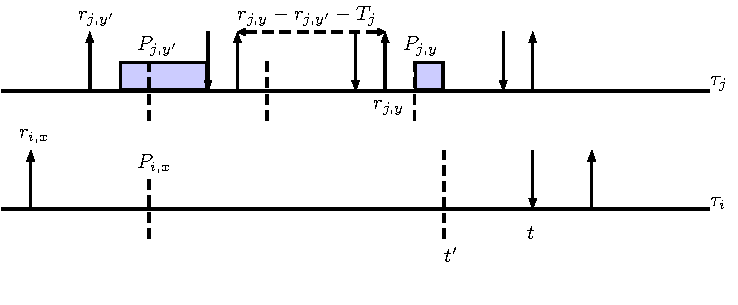
\includegraphics[scale=0.7]{fig/Cy}  
\caption{$D_j-p_j<C_j$}
  \label{fig:o2}
\end{figure}
With the above lemma, we have
	\begin{align*}
	\begin{split}
	g_{i}(\tau_j,t',t)=
	\begin{cases}
	&\min(D_j-p_j, t'-P_{i,x})~\mbox{~~~~~if~} y=y'\\
	&D_j-p_j+\frac{r_{j,y}-r_{j,y'}-T_j}{T_j}(D_j-p_j)\\&+\min(D_j-p_j, [t'-P_{j,y}]_0)\mbox{~otherwise} \\
	\end{cases}
	\end{split}
	\end{align*}

% \subsection{Optimized test}
Since total execution before $P_{i,x}$ (if $t'>P_{i,x}$) is bounded by  $P_{i,x}$, we can use a simple optimization technique to further tighten the test. Therefore we have 

\begin{equation}
\begin{split}
F_i(\tau,t',t)=~~~~~~~~~~~~~~~~~~~~~~~~~~~~~~~~~~~~~~~~~~~~~~\\
\begin{cases}
& \sum\limits_{\tau_j\in\{\tau\setminus\tau_i\}}f_i(\tau_j,t',t)+ \lfloor \frac{t-D_i}{T_i} \rfloor C_i\mbox{~If~} t'\leq P_{i,x}\\
&\min\!\left(P_{i,x},  \lfloor \frac{t-D_i}{T_i} \rfloor C_i\!\!+\!\!\!\!\!\!\!\sum\limits_{\tau_j\in\{\tau\setminus\tau_i\}}\!\!\!\!\!\!f_i(\tau_j,t',t)\!-\!g_{i}(\tau_j,t',t)\!\right)\\&+\sum_{\tau_j\in\{\tau\setminus\tau_i\}}g_{i}(\tau_j,t',t)\mbox{~~~~~~~~~~~~~Otherwise}
\end{cases}	
\end{split}
\end{equation}





\subsection{Upper bound of $t$}

We also need to derive an upper bound of $t$ because otherwise $t$ can tends to infinity. Suppose there exists a $t$ so that
\begin{align*}
\forall~t'\in(t-D_i,t]:~F_i(\tau,t,t')+C_i>t'\\
\Rightarrow\min_{t'\in(t-D_i,t]}\frac{F(\tau_i,t,t')+C_i}{t'}>1	
\end{align*}

, and let
\begin{align*}
H_i(t)= & U\times t+\sum_{\tau_j\in\{\tau\setminus\tau_i\}}C_j+C_i\\&\geq t\times u_i+\sum_{\tau_j\in\{\tau\setminus\tau_i\}}(\lfloor \frac{t'}{T_j} \rfloor+1)C_j+C_i\\
&\geq F(\tau_i,t,t')+C_i
\end{align*}
Then it must be that

\begin{align*}
&\frac{H_i(t)}{t-D_i}>1\Rightarrow t-D_i< U\times t+\sum_{\tau_j\in\{\tau\setminus \tau_i\}}C_j+C_i\\
&\Rightarrow t<\frac{D_i+\sum_{\tau_j\in\tau\setminus \tau_i}C_j+C_i}{1-U}
\end{align*}

\subsection{Promotion Point Tuning}
The promotion point of each task has a great influence on the schedulability of the system. In this section we propose a promotion point tuning algorithm to find  suitable promotion point for each task. The system $\tau$ will have an initial promotion point assignment based on the principle that: a task with lower origin priority has an shorter promotion point so that it can enter promotion stage earlier. Such a promotion point assignment principle enhances the chances that each task can complete by  deadline.

Thus here we this the following initial promotion point policy.
\begin{equation}
p_i=T_i-C_i-\sum\limits_{j<i}C_j
\end{equation}
This assignment policy in fact is optimal when the system comprises of two tasks. Once our test detects $\tau_i$ has a deadline miss at $t$, then its promotion point decreases by $dec_i$ until $p_i$ decreases to $0$. The value of $dec_i$ controls the speed of the test because in the worst cases we may need to try all the possible combinations of $p_i$.  Thus here we ensure $dec_i$ fall in the range $[\delta_i^{min},\delta_i^{max}]$ so that the value of $dec_i$ is neither too large nor too small. On the other hand $J_{j,y}$~($j>i$) can only interfere $J_{i,x}$ only if $P_{j,y}<P_{i,x}$, and $J_{j,y}$~($j<i$) can not interfere $J_{i,x}$ during $[P_{i,x},P_{j,y}]$. Therefore we can record 
\[\delta_i=\min\limits_{\tau_j\in\tau\setminus \tau_i\wedge P_{i,x}>P_{j,y} }P_{i,x}-P_{j,y}\]
, and once we detects that $\tau_i$ is not schedulable, 
\[
p_i=p_i-\min\left(\delta_i^{max} \max\left(\delta_i^{min},\delta_i\right)\right)
\]

In sum the detailed steps of the promotion point tuning steps are presented in the following algorithm.
\begin{algorithm}
   \caption{Promotion Point Tuning}
    \begin{algorithmic}[1]
      \Function{PP\_T}{$\tau$}
        \While{flag == TRUE}
        \State flag$\leftarrow$ FALSE
        \For{$\tau_i\in \tau$}
		\If {TEST($\tau_i,\tau$)==FALSE}
			\If {$p_i>dec_i$}
			\State $p_i\leftarrow p_i-\min\left(\delta_i^{max} \max\left(\delta_i^{min},\delta_i\right)\right)$
			\State flag$\leftarrow$ TRUE
			\State Break
			\Else
			\State \Return FALSE
			\EndIf
		\EndIf
        \EndFor
		\EndWhile
		\State \Return TRUE
     
       \EndFunction
      	\Function{test}{$\tau_i,\tau$}
	  	\State flag = TRUE
      	\For{$t\in [D_i,t^{max}]$}
				\For{$t'\in [t-D_i,t]$}
			    	\If {$F_i(\tau,t',t)\leq t'$}
						\State flag$\leftarrow$ TRUE
						\State Break
					\EndIf
				\EndFor
				\If {flag==FALSE}
					\Return FALSE
				\Else
					\State flag$\leftarrow$ FALSE
				\EndIf

			\EndFor
				\State \Return TRUE
		\EndFunction
\end{algorithmic}
\end{algorithm}

% \section{Draft Simulation Results}

% \begin{table}[h]
% \caption{Notations}
% \label{tab:x}
% \large
% \center
% \begin{tabular}{|l|l|l|l|l|}
%  \hline
% Uniform Distribution&[0.88,0.9]&[0.93,0.95]&[0.95,0.97]&[0.97,0.99]\\
%  \hline
% Acceptance Ratio&1&1&0.995&0.982\\
%  \hline
% \end{tabular}
% \end{table}